% Teori

\chapter{Teori} % Chapter title

\label{ch:teori} % For referencing the chapter elsewhere, use \autoref{ch:mathtest}

% Formålet med dette kapittelet er å gjøre rede for tidligere arbeid innenfor fagfeltet og samle bakgrunnsinformasjon som er nødvendig for å forstå det arbeidet som utføres i oppgaven. Kapittelet inneholder
% fagrelatert informasjon og tekniske begreper som brukes i løsning og implementasjon.
%----------------------------------------------------------------------------------------

\section{Pioneer P3-DX}

Pioneer P3-DX er en robot levert av Adept MobileRobots. Den er sett på som pålitelig, og derfor ofte brukt i forbindelse med forskning og eksperimenter. Roboten kommer som standard med to styrbare 19 cm hjul, et lite, passivt støttehjul, og 8 sonarsensorer montert foran, og tilsvarende bak. I tillegg er det på utgaven som ITK besitter montert et forriglingssystem i form av kontaktsensorer, også kalt <<bumper>>-sensorer, langs hele kanten foran og bak. På toppen av roboten er det en flat plattform, perfekt for montasje av annet utstyr. 

Roboten har en egen innebygget kontroller for styring, tilgjengelig via seriellport. For å kontrollere roboten via ROS benyttes det en driver som sender kommanodoer til robotens grensesnitt, ARIA\footnote{\url{http://robots.mobilerobots.com/wiki/ARIA}}. ARIA, eller Advanced Robot Interface for Applications, lar brukeren kontrollere robotens fart og retning, lese av sensorverdier og så videre.

\begin{figure}[h!]
  \centering
    \reflectbox{%
      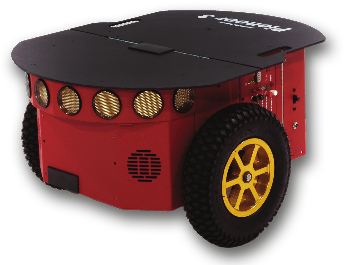
\includegraphics[width=0.5\textwidth]{gfx/pioneer3dx_real.png}}
  \caption{Pioneer P3-DX}
  \label{fig:pioneer}
\end{figure}

\section{ROS}

ROS (Robot Operating System) er et fleksibelt rammeverk for styring av roboter. Rammeverket har fokus på brukervennlighet og robusthet, og er ikke spesifikt for én type robot. ROS har derfor gjort seg svært egnet for dette prosjektet. Operativsystemet er bygget opp av moduler som sender og mottar informasjon via meldingskanaler. Dette letter implementasjon av de enkelte modulene, da de får tydelige grensesnitt som gjør at de kan testes uavhengig av andre moduler.

\section{Flex 13 og Motion Capture Systems}

Flex 13 er et infrarødt kamera, levert av OptiTrack\footnote{\url{https://www.optitrack.com/}}. Markører, i form av kuler med en spesiell overflate, reflekterer de infrarøde strålene tilbake slik at de oppdages av kameraet. Ved å lage bestemte mønstre med slike kuler, og bruke samme type kamera i forskjellige vinkler er det mulig å danne svært nøyaktige tredimensjonale inntrykk av fysiske objekter. Et slikt system er et eksempel på et <<Motion Capture System>>, og da brukes det til å spore bevegelsene til objekter. Data fra et slik system kan brukes til mange forskjellige formål, og avhenger helt av kompleksiteten til objektet som spores. 


% Et  «Motion  Capture»  system  har  blitt  brukt  som  posisjoneringssys-tem for dette prosjektet. Kamerasystemet består av rekke takmontereinfrarøde kamera som er i stand å fange opp refleksjoner fra spesiellemarkører nede på bakken. Ved bruk av skreddersydd programvare erdette systemet i stand til å kalkulere kartesiske koordinater med millimeterpresisjon for de gitte markørene og sende disse koordinatene utpå en strøm. 


\section{Motive}

Motive er en programvare pakke fra OptiTrack. Programmet henter data fra de infrarøde kameraene, og presenterer et tredimensjonalt bilde over markørene som befinner seg innenfor kameraenes synsområde.
Disse kan grupperes og defineres som legemer, og programmet kan deretter spore både posisjon og orientasjon for hvert legeme. Bevegelsene til legemene kan lagres for senere analyse, eller de kan overføres 
til andre datamaskiner på nettverket.

\section{Stifinning}

Stifinning er tilnærmingen på å finne korteste vei fra ett punkt til et annet. Det er mange måter å gjennomføre dette på, og avhenger helt av miljøet hvor det skjer og hvilke data som er og blir tilgjengelig. Et praktisk problem kan f.eks. være å sammenlikne forskjellige ruter for en bil som skal frakte varer fra by A til by B. Basert på kunnskap om fartsgrenser og avstander vil en algoritme kunne hvilke noder bilen må kjøre om for å komme dit på kortest mulig tid.

Én av de mest kjente algoritmene for dette formålet er Dijkstras algoritme. 



\section{SLAM}

SLAM, eller Simultaneous Localization and Mapping, tar for seg problemet med å navigere i ukjente omgivelser, samtidig som man kartlegger omgivelsene. SLAM består i flere steg. Roboten mottar oppdateringer fra interne og eksterne sensorer slik som GPS og akselerometer, og kombinerer dette ved hjelp av et utvidet Kalmanfilter. Roboten scanner området rundt seg, med en laser eller på annen måte, og identifisere landemerker. Roboten vil deretter bruke denne informasjonen til å korrigere for usikkerheten i de andre sensorene, samtidig som den konstruerer et kart over omgivelsene. \cite{slam_for_dummies}